\begin{figure}[h!]
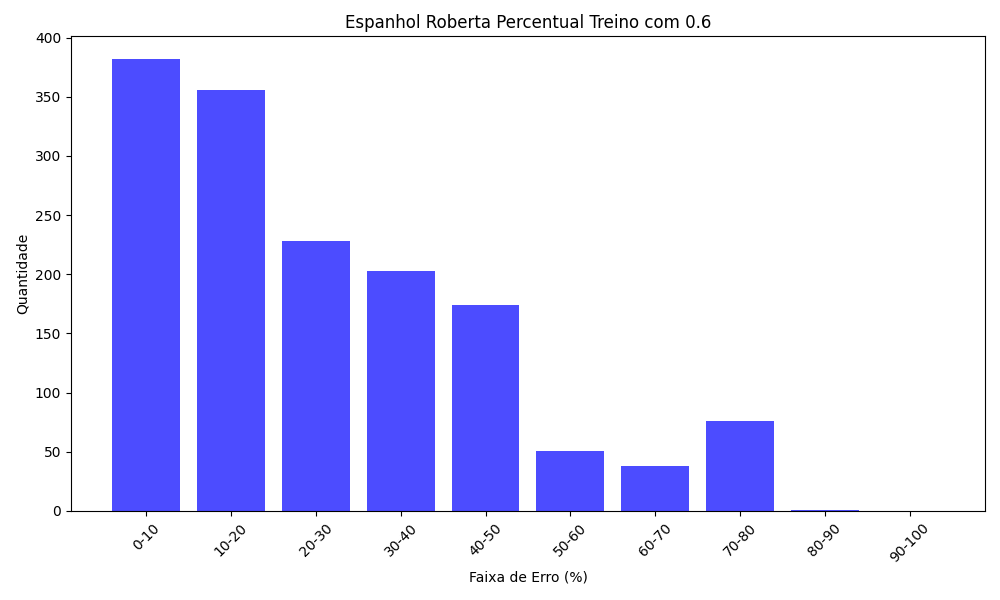
\includegraphics[width=\textwidth]{img/grafsEsp/Espanhol Roberta Percentual Treino com 0.6_quantidade.png}
\caption{Quantidade de respostas por faixas de erro percentual dos testes com 40\% do \textit{dataset} (Modelo Espanhol \textit{ROBERTA})}\label{figure:12}
\end{figure}

\begin{figure}[h!]
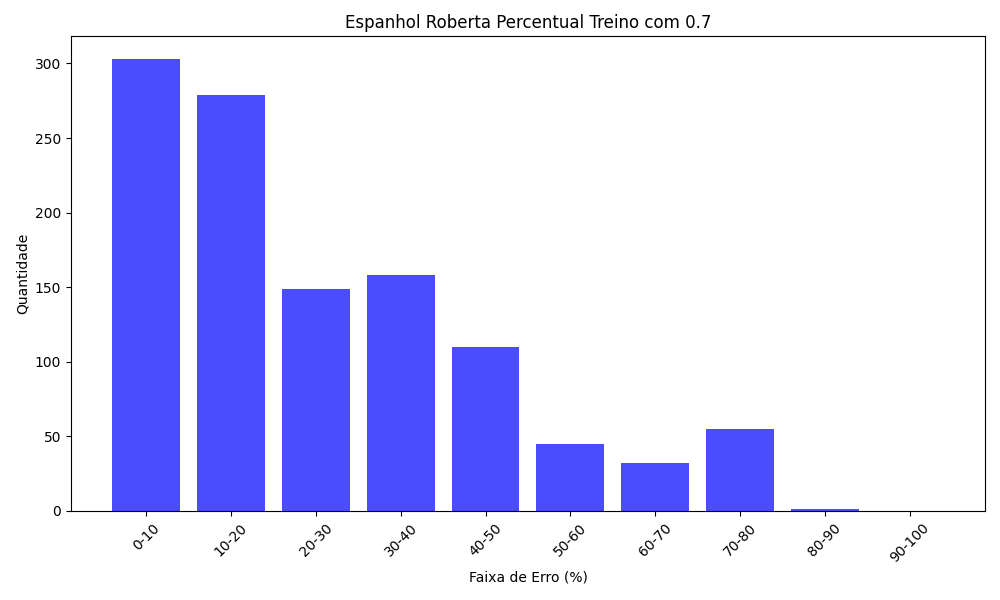
\includegraphics[width=\textwidth]{img/grafsEsp/Espanhol Roberta Percentual Treino com 0.7_quantidade.png}
\caption{Quantidade de respostas por faixas de erro percentual dos testes com 30\% do \textit{dataset} (Modelo Espanhol \textit{ROBERTA})}\label{figure:13}
\end{figure}

\begin{figure}[h!]
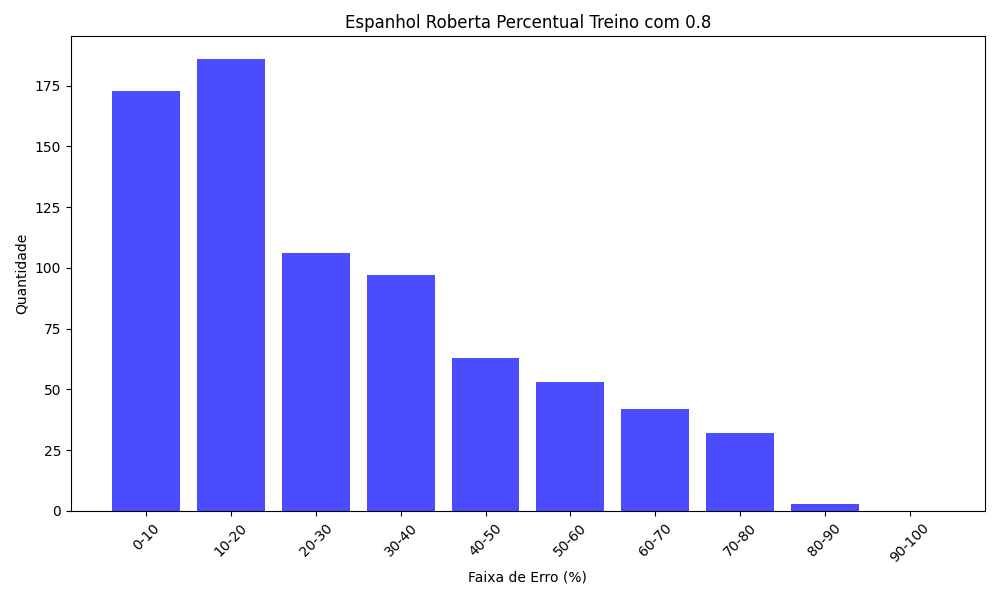
\includegraphics[width=\textwidth]{img/grafsEsp/Espanhol Roberta Percentual Treino com 0.8_quantidade.png}
\caption{Quantidade de respostas por faixas de erro percentual dos testes com 20\% do \textit{dataset} (Modelo Espanhol \textit{ROBERTA})}\label{figure:14}
\end{figure}

\begin{figure}[h!]
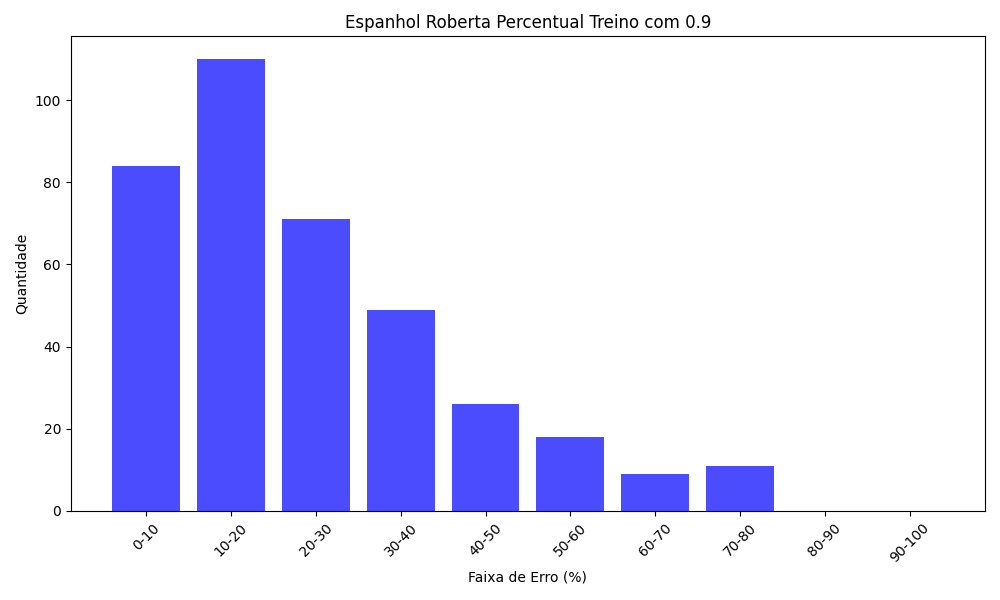
\includegraphics[width=\textwidth]{img/grafsEsp/Espanhol Roberta Percentual Treino com 0.9_quantidade.png}
\caption{Quantidade de respostas por faixas de erro percentual dos testes com 10\% do \textit{dataset} (Modelo Espanhol \textit{ROBERTA})}\label{figure:15}
\end{figure}